\newcommand{\alphainv}{\alpha^{-1}}

\section{Definitions}

\begin{definition*}[Group]
  A group is a set, together with a binary operation that maps any two elements
  to another element in the set. I.e. it is a triple $(S, \cdot, I)$ specifying
  the set, the operation and the identity element respectively. It satisfies the
  group axioms:
  \begin{enumerate}
  \item existence of identity
  \item existence of an inverse for each element
  \item associativity
  \end{enumerate}
  If the operation is commutative it is said to be ``abelian''.
\end{definition*}

\begin{definition*}[Homomorphism]
  A structure-preserving map between two groups
\end{definition*}

\begin{definition*}[Endomorphism]
  A homomorphism from a group to itself.
\end{definition*}

\begin{definition*}[Field]
  A field is a set $\F$ for which both $(\F, +, 0)$ and $(\F, \times, 1)$ are abelian groups.
\end{definition*}

\begin{definition*}[Vector space]
  A vector space $V$ over a field $\F$ is an abelian group $(V, +, 0)$ for which
  multiplication by ``scalars'' from $\F$ is defined, and additionally satisfies
  \begin{enumerate}
  \item Linear combinations using scalars from $\F$ remain within the vector
    space:\\
    $au + bv \in V$ for all $a, b \in \F$ and $u, v \in V$.
  \end{enumerate}
\end{definition*}

\begin{definition*}[Ring]\footnote{Gross, Abstract Algebra, lecture 24}
A ring is an abelian group $(R, +, 0)$ which additionally has a multiplication
operation. The multiplication may or may not be commutative, and does not
necessarily have inverses. Both distributive laws must hold unless we're
assuming commutativity: $a(b + c))$ and $(b + c)a$.
\end{definition*}

\subsubsection{Examples}
\begin{itemize}
\item zero ring $\{0\}$ (multiplicative identity is $1 = 0$ in this ring; in
  any other ring $1 \neq 0$.)
\item Any field is a ring
\item $\Z$
\item $\Z/n\Z$
\item Set of $n \times n$ matrices over a field
\end{itemize}

Subrings must contain $0, 1$.

Subring of $\C$: Gaussian integers $\Z + i\Z$.

What about sets of lines through the origin in complex plane such that angles
are closed under addition? That's a subring of $\C$ too right?

``Best way to get rings'': \textbf{endomorphism ring}. Start with an abelian
group $(A, +, 0)$. The endomorphism ring is the set of all group homomorphisms
$A \to A$ \footnote{aren't these called automorphisms?}
\begin{align*}
\End(A) = \{f: A \to A\}
\end{align*}
Addition and multiplication are defined by
\begin{align*}
  (f + g)(a) &= f(a) + g(a)\\
  (fg)(a)    &= f(g(a)).
\end{align*}
It must have an additive identity. This must be the constant zero function
$0(a) = 0$. Is that a homomorphism? Yes: $0(a + b) = 0 = 0(a) + 0(b)$.

And additive inverse: $(-f)(a) = -(f(a))$. Is that a homomorphism? Yes:
\begin{align*}
  (-f)(a + b) = -(f(a + b)) = -(f(a) + f(b)) = -f(a) + -f(b)
\end{align*}

The multiplicative identity is just the identity homomorphism.

Multiplication (i.e. composition) is not necessarily commutative.

It would be a field if there were multiplicative inverses: do these exist? Only
for those homomorphisms that are isomorphisms.

To construct the ring $\Z$: it's (isomorphic to) the endomorphism ring of the
group $(\Z, +, 0)$. What's the correspondence between group homomorphisms and
integers? Well, consider group homomorphism $f$. The entire homomorphism is
determined by $f(1)$! Since
\begin{align*}
  f(1) &= k\\
  f(2) &= f(1 + 1) = f(1) + f(1) = 2k\\
       \ldots\\
  f(n) &= kn.
\end{align*}
So we map the homomorphism $f$ to the integer $f(1)$.

And if $f(1) = k_1$ and $g(1) = k_2$, then multiplication of integers is
\begin{align*}
  (f \times g)(n) = f(g(n)) = k_1k_2n.
\end{align*}
This is the reason why the product of two negative integers is positive: a
negative number corresponds to a homomorphism that maps positive integers to
negative.

Similarly,
\begin{align*}
  \Z/n\Z = \End(\Z/n\Z, +, 0)
\end{align*}
since we identify $1$ with...

This is a phenomenon of cyclic groups. I.e. $\Z/n\Z$ (finite) and $\Z$
(infinite). There are no other cyclic groups.

\subsection{Polynomial}

A polynomial is $P(x) = a_0 + a_1x^1 + \ldots + a_nx^n$.

The coefficients $a_i$ must come from some ring $R$, and the set of all such
polynomials is written $R[x]$.

If $R$ is a commutative ring, so is $R[x]$.

Therefore we can write a polynomial in two variables as $R[x][y]$, i.e. the
coefficients of the polynomial in $y$ are themselves polynomials in $x$.

If $R = \C$ this leads towards algebraic geometry. Rings like integers,
Gaussian integers, etc are the subject of number theory.

The variable/``indeterminate'' $x$ must also come from some ring, since it is
involved in both addition and multiplication (?).

Multiplication of polynomials e.g. coefficients from $R = \Z/2\Z$:
\begin{align*}
(x + 1)(x + 1) = x^2 + 2x + 1 = x^2 + 1
\end{align*}
since $2 = 0 \mod 2$.

\section{Vector Spaces}

\subsection{Definitions}

\subsubsection{Linear independence}
A set of vectors $\{v_1, v_2, \ldots\}$ are linearly independent if the only
solution to
\begin{align*}
  a_1v_1 + a_2v_2 + \ldots = 0
\end{align*}
is $a_1 = a_2 = \ldots = 0$.


\subsubsection{Span}
The span of a set of vectors is the set of all vectors that can be formed from
them by linear combination.


\subsubsection{Basis}
$E \subset V$ is a basis for $V$ if
\begin{enumerate}
\item $E$ spans $V$
\item if the addition of any further $v \in V\setminus E$ to $E$ would cause
  $E$ to lose its linear dependence.
\end{enumerate}


\subsubsection{Coordinates}
The coordinate of a vector $v$ in basis $E = \{e_1, e_2, \ldots, e_n\}$ is the
unique list of scalars $a_1, a_2, \ldots, a_n$ such that
$v = a_1e_1 + a_2e_2 + \ldots + a_ne_n$.

So although a vector $v$ may live in an $n$-dimensional space, $v$ does not
consist of a list of $n$ components until it is represented by its coordinates
in a particular basis.


\subsubsection{Linear transformation}
A linear transformation $f: V \to W$ is a homomorphism between the vector
spaces, preserving linear transformation: for $u, v \in V$
\begin{align*}
  f(au + bv) = af(u) + bf(v).
\end{align*}

Having fixed a basis $E$ for $V$, to specify $f$ it's sufficient to specify
$f(e)$ for all $e \in E$. That's what a matrix is: it contains $f(e_j)$ in
column $j$.


\subsection{The space of functions $f:\N \to \R$}

The elements of the vector space are functions (i.e. subsets of $\N \times \R$).

(They are sequences.)

This is a group under addition of functions: $f + g: \N \to \R$ where
$(f + g)(n) = f(n) + g(n)$. The identity is the zero function $f(n) = 0$.

So we have addition of functions, but multiplication of functions plays no
role. Is the set of all functions a field?


The vector space is over a field, say $\R$. For $a \in \R$, $(af)(n) = a(f(n))$.

Once we have established a basis $E$, then each function can be assigned
numerical coordinates in the (infinite-dimensional) vector space.

So what would be a basis for this vector space?




\newpage
\section{Groups}

Consider a set $A$ with $n$ elements.

\begin{definition*}
  A \textbf{permutation} is a bijection: $A \to A$. There are $n!$ permutations of $A$.
\end{definition*}

\begin{definition*}
  The \textbf{symmetry group} $S_n$ is the set of permutations of a set of size $n$, denoted
  $S_n = \Sym(\{1,2,\ldots,n\})$. It is a group, under composition.
\end{definition*}

\begin{definition*}
  Consider an $n$-sided regular polygon. A \textbf{symmetry} of the polygon is an isometry of the
  plane which preserves the polygon.
\end{definition*}

\begin{definition*}
  The \textbf{dihedral group}
  $D_{2n}$ is the group of symmetries under composition. It is of order $2n$. Let
  $r$ be a clockwise rotation through $360/n$ degrees, and let $s$ be a
  reflection about a chosen axis of symmetry. The elements of the group are
  \begin{align*}
    e, r, r^2, \ldots, r^{n-1}, s, sr, sr^2, \ldots, sr^{n-1}.
  \end{align*}
\end{definition*}

\begin{remark*}
  The symmetry group contains permutations; some of these are not symmetries.

  The set of symmetries is a proper subset of the set of permutations of the vertices: for example
  the permutation which interchanges two adjacent vertices but leaves all other vertices unchanged
  is not a symmetry.
\end{remark*}

\begin{intuition*}
  A $k$-\textbf{cycle} is a permutation that cycles $k$ elements and leaves the rest unchanged. Its
  order is $k$.
\end{intuition*}

\begin{definition*}
  A permutation $\sigma \in S_n$ is a $k$-\textbf{cycle} if there exist $k$ distinct elements
  $a_1, \ldots, a_k \in S_n$ such that
  \begin{align*}
    \begin{cases}
      a_i\sigma = a_{i+1} \text{~for~} 1 \leq i < k\\
      a_k\sigma = a_1\\
      x\sigma = x \text{~for~} x \notin \{a_1, \ldots, a_k\}.
    \end{cases}
  \end{align*}
  The cycle $\sigma$ is written as e.g. $(a_1, a_2, \ldots, a_k)$, but note that e.g.
  $(a_2, a_3, \ldots, a_k, a_1)$ is the same thing.
\end{definition*}

\begin{example*}
  Let
  \begin{align*}
    \alpha =
    \begin{pmatrix}
      1 & 2 & 3 & 4 & 5\\
      2 & 4 & 3 & 1 & 5
    \end{pmatrix}
                      ~~~
                      \beta =
                      \begin{pmatrix}
                        1 & 2 & 3 & 4 & 5\\
                        3 & 4 & 5 & 1 & 2
                      \end{pmatrix}
                                        ~~~
                                        \gamma =
                                        \begin{pmatrix}
                                          1 & 2 & 3 & 4 & 5\\
                                          2 & 5 & 4 & 3 & 1.
                                        \end{pmatrix}
  \end{align*}
  Determine the product $\alpha\beta\gamma$, the inverse of $\beta$ and the order of $\gamma$.

  In cycle notation,
  \begin{align*}
    \alpha = (124) ~~~ \beta = (13524) ~~~ \gamma = (125)(34).
  \end{align*}

  By following each element in turn through the 3 permutations (using either representation),

  \begin{align*}
    \alpha\beta\gamma =
    \begin{pmatrix}
      1 & 2 & 3 & 4 & 5\\
      3 & 2 & 1 & 4 & 5
    \end{pmatrix} = (13).
  \end{align*}

  \begin{align*}
    \beta^\1 =
    \begin{pmatrix}
      3 & 4 & 5 & 1 & 2\\
      1 & 2 & 3 & 4 & 5
    \end{pmatrix}
                      =
                      \begin{pmatrix}
                         1 & 2 & 3 & 4 & 5\\
                         4 & 5 & 1 & 2 & 3
                      \end{pmatrix}
                                         = (14253).
  \end{align*}

  The order of $\gamma$ is 6.
\end{example*}

\section{Examples of groups, homomorphisms and quotients}

\subsection{Finite order}

\begin{itemize}
\item $S_2$: the set of permutations of two objects, where the operation is
  composition of functions.  There are just two elements in the group: the
  do-nothing permutation and the switch-the-elements permutation: $\{e,
  \tau\}$.

\item $S_3 \cong D_3$: the symmetry group $S_3$ is the set of permutations of three objects. There
  are 6 elements: the identity, 3 transitions\footnote{A transition is a permutation that switches
    two elements and leaves all other alone} and two cyclic permutations. It's isomorphic to the
  dihedral group $D_3$, i.e. the group of symmetries of an equilateral triangle: the two cyclic
  permutations correspond to rotation by $\pi/3$ and $2\pi/3$ radians, and the three transitions
  correspond to the 3 possible reflections (each of which leaves one vertex unchanged).
  \begin{mdframed}
    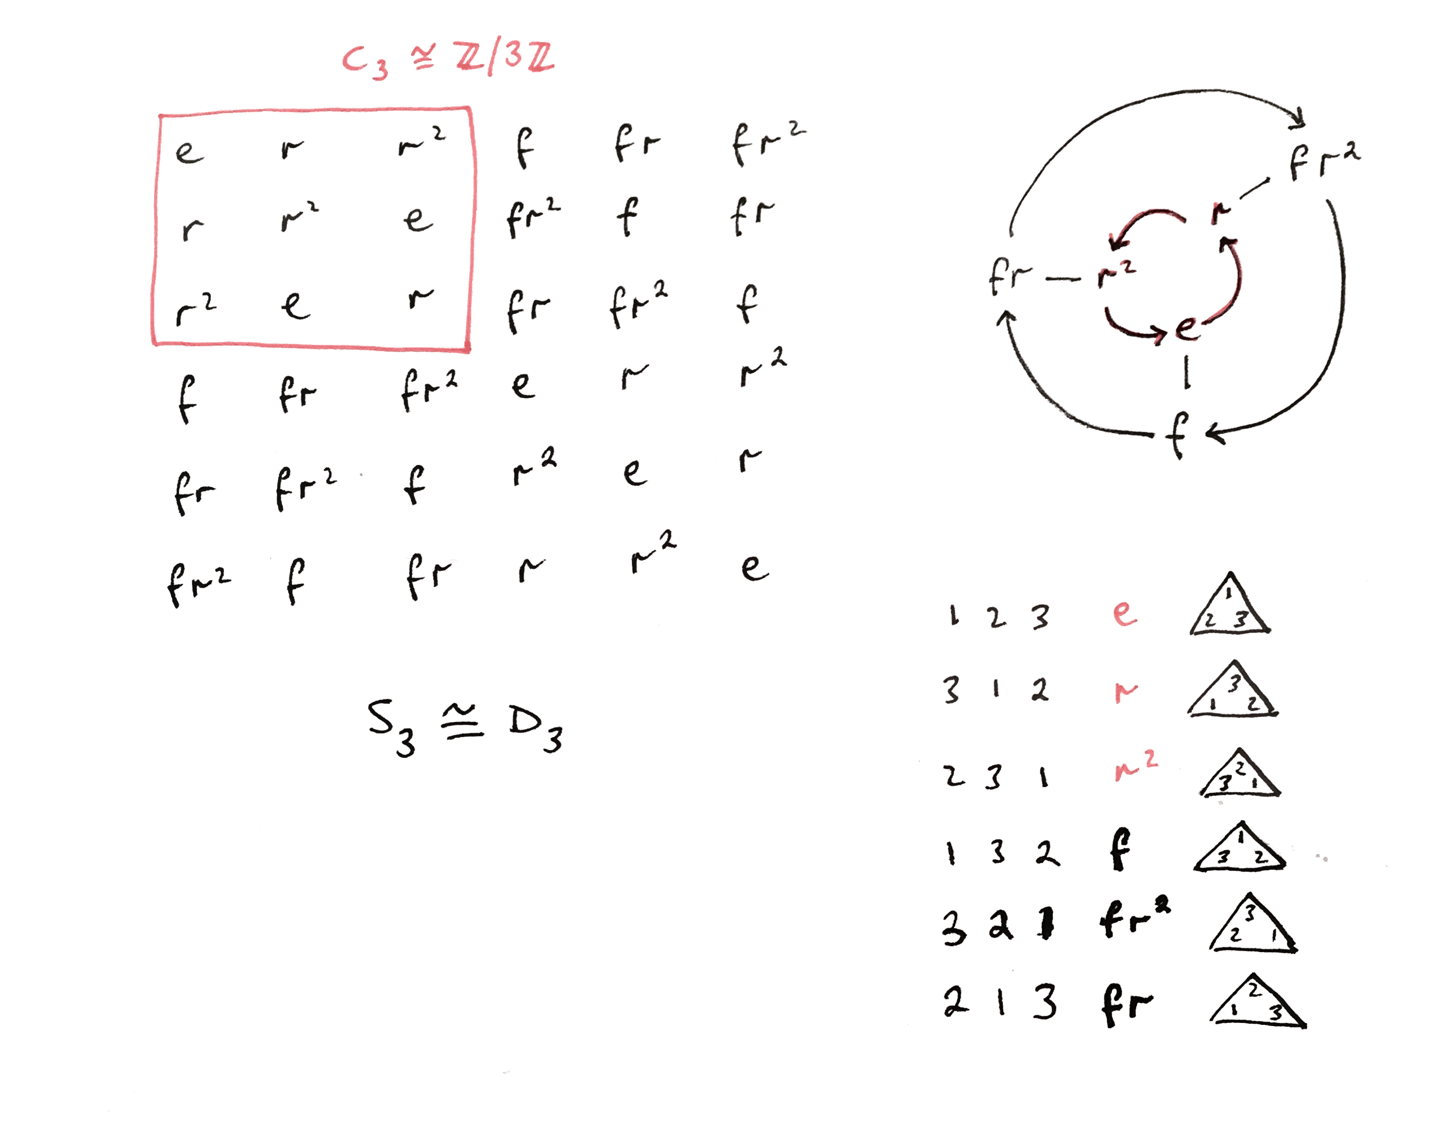
\includegraphics[width=400pt]{img/abstract-algebra-s3-d3.png}
  \end{mdframed}
\item $\{1, i, -1, -i\}$ where the operation is multiplication of complex numbers.
\end{itemize}

\subsection{Infinite order}

\begin{itemize}
\item The group $\Z$, i.e. integers under addition
  \begin{itemize}
  \item[$\diamond$] A homomorphism is $f:\Z \to \{0, 1\}$, given by $f(n) =
    \begin{cases}
      0, ~~\text{$n$ is even}\\
      1, ~~\text{$n$ is odd}\\
    \end{cases},$ with the operation on $\{0, 1\}$ being addition mod 2. The kernel is
    $evens = 2\Z$, and the resulting quotient group is
    $\Z/2\Z = \{evens, odds\} = \{2\Z, 2\Z + 1\}$.
  \end{itemize}

\item The ring $\Z$ - example of homomorphism.
\item $\Z_{>0}^+$ positive integers under addition

\item Similarly, $\Q^+$, $\Q^\times$, $\C^+$, $\C^x$, $\R^+$, $\R^x$ etc

\item $GL_n(\F)$: the set of $n \times n$ matrices with entries from the field $\F$, under matrix
  multiplication.
  \begin{itemize}
  \item[$\diamond$] A homomorphism is $f:GL_n(\F) \to \F^\times$ given by $A \mapsto \det(A)$. This
    is a homomorphism since $\det(AB) = \det(A) \det(B)$. The kernel is the set $SL_n(\F)$ of
    matrices with determinant 1. If the field is $\R$ then these rotate or flip space without
    stretching it. The resulting quotient group is the set $\{\mathcal{A}(x) ~|~ x \in \F\}$, where
    $\mathcal{A}(x)$ is the set of matrices with determinant $x$.
  \end{itemize}

\item The set $\F[x]$ of polynomials with coefficients in a field $\F$ can be a vector space, and a
  ring. (Not a field, since multiplicative inverses don't exist for degree $\geq 1$.)

  As a vector space, differentiation is a linear transformation (homomorphism). This is
  non-injective (polynomials differing only by an additive constant additive are sent to the same
  polynomial). The kernel is the set of degree 0 polynomials ($\F$). The quotient space $\F[x]/\F$
  contains cosets of the form $p(x) + \F$, i.e. a set of polynomials differing only by an additive
  constant.

  But differentiation does not preserve multiplication of polynomials, so it is not a ring
  homomorphism.

\item $SL_n(\R)$: set of $n \times n$ matrices with determinant $1$ (kernel of the
  determinant homomorphism $GL_n(\R) \rightarrow \R^\times$ and therefore a normal
  subgroup of $GL_n(\R)$)
\end{itemize}


\newpage
\section{Homomorphism}

A \textbf{homomorphism} is a map from one group to another. If it is bijective,
it is an \textbf{isomorphism}. If it is bijective and from a group to itself
(i.e. a permutation of the group elements) then it is an
\textbf{automorphism}. The critical feature of these concepts is that they
``preserve group structure'', i.e. they preserve the relationships among group
elements defined by the group operation. Suppose that they map from group $G$
to group $G'$. Then the preservation-of-structure criterion is that the map
sends a product $g_1 \circ g_2$ to the product of whatever the separate
elements are sent to:

$$
f(g_1 \circ g_2) = f(g_1) \circ f(g_2)
$$

There the composition on the left is happening in $G$ and the composition on
the right is happening in $G'$. (For an automorphism, $G=G'$.)

Another way of saying this is that ``the following diagram commutes'':
\begin{align*}
  \matMMMxNNN
  {g_1, g_2}{\xrightarrow{~~f~~}}{f(g_1), f(g_2)}
  {\Big\downarrow}{}{\Big\downarrow}
  {g_1g_2}{\xrightarrow{~~f~~}}{f(g_1g_2) = f(g_1)f(g_2)},
\end{align*}
i.e. it does not matter whether you first perform the internal structure operation on the left-hand
side and then apply $f$, or alternatively apply $f$ first and perform the internal structure
operation on the right-hand side.

Note that an element such as $g_1$ that is being sent somewhere by a morphism
may itself already be a map of sorts, e.g. if it is a permutation in
$S_3$. This is potentially confusing, since an automorphism can be thought of
as a permutation of group elements. So an automorphism on $S_3$ is a
permutation of group elements that are themselves permutations of some generic
labeled objects.

The definition of homomorphism implies that $f(g^{-1}) = f(g)^{-1}$ since
$f(gg^{-1}) = f(g)f(g^{-1}) = f(e)$.

\section{Kernel, Nullspace, Bijection and Congruency}

Consider a homomorphism $f$ with kernel $N$.

\textbf{Theorem:} $a$ and $b$ are sent to the same place by $f$ if and only if
$b = an$ for some $n \in N$.

\textbf{Corollary:} $f$ is a bijection (isomorphism) if and only if the kernel
contains only the identity element.

\textbf{Example:} Consider the absolute value homomorphism mapping complex numbers
under multiplication to positive reals under multiplication. The equivalence
classes are concentric circles around the origin. Two complex numbers have the
same absolute value iff one can be obtained from the other by rotation only (no
scaling). This is multiplication by a complex number with absolute value 1, and
such a complex number is in the kernel.

\textbf{Proof:} Clearly, if $b = an$ then $b$ is sent to the same place as $a$,
since

$$
f(b) = f(an) = f(a)f(n) = f(a).
$$

However we need to demonstrate the converse, i.e. that the *only* way that $b$
can be sent to the same place as $a$ is if $b=an$ for some $n \in N$.

Two almost identical ways of showing that:

\textbf{(1) Show that if $f(a) = f(b)$ then $b = an$ for some $n \in N$}

In linear algebra, you can always get from $u$ to $v$ by adding $v - u = -u +
v$, so the claim is that $L(u) = L(v)$ implies $-u + v$ is in the nullspace,
which is true:

$$
L(-u + v) = L(-u) + L(v) = L(-u) + L(u) = 0.
$$

For a group homomorphism, $b$ can be written as $aa^{-1}b$, so the claim is
that $f(a) = f(b)$ implies $a^{-1}b \in N$, which is true:

$$
f(a^{-1}b) = f(a^{-1})f(b) = f(a)^{-1}f(a) = e.
$$

\textbf{(2) Show that if it is not the case that $b = an$ for some $n \in N$, then $f(a) \neq f(b)$}

In linear algebra, you can always get from $u$ to $v$ by adding $v - u = -u + v$,
so if $-u + v$ is not in the nullspace then

$$
L(v) = L(u + (-u + v)) = L(u) + L(-u + v) \neq L(u).
$$

For a group homomorphism, $b$ can be written as $aa^{-1}b$, so if $a^{-1}b$ is
not in the kernel then

$$
f(b) = f(aa^{-1}b) = f(a)f(a^{-1}b) \neq f(a)
$$


\section{Inverse of an automorphism is an automorphism}

[Artin 2.3.11: show that Aut($G$) is a group]

Suppose $\alpha$ is an automorphism that sends $g_1$ and $g_2$ to $g_1'$ and
$g_2'$, respectively.

\begin{mdframed}
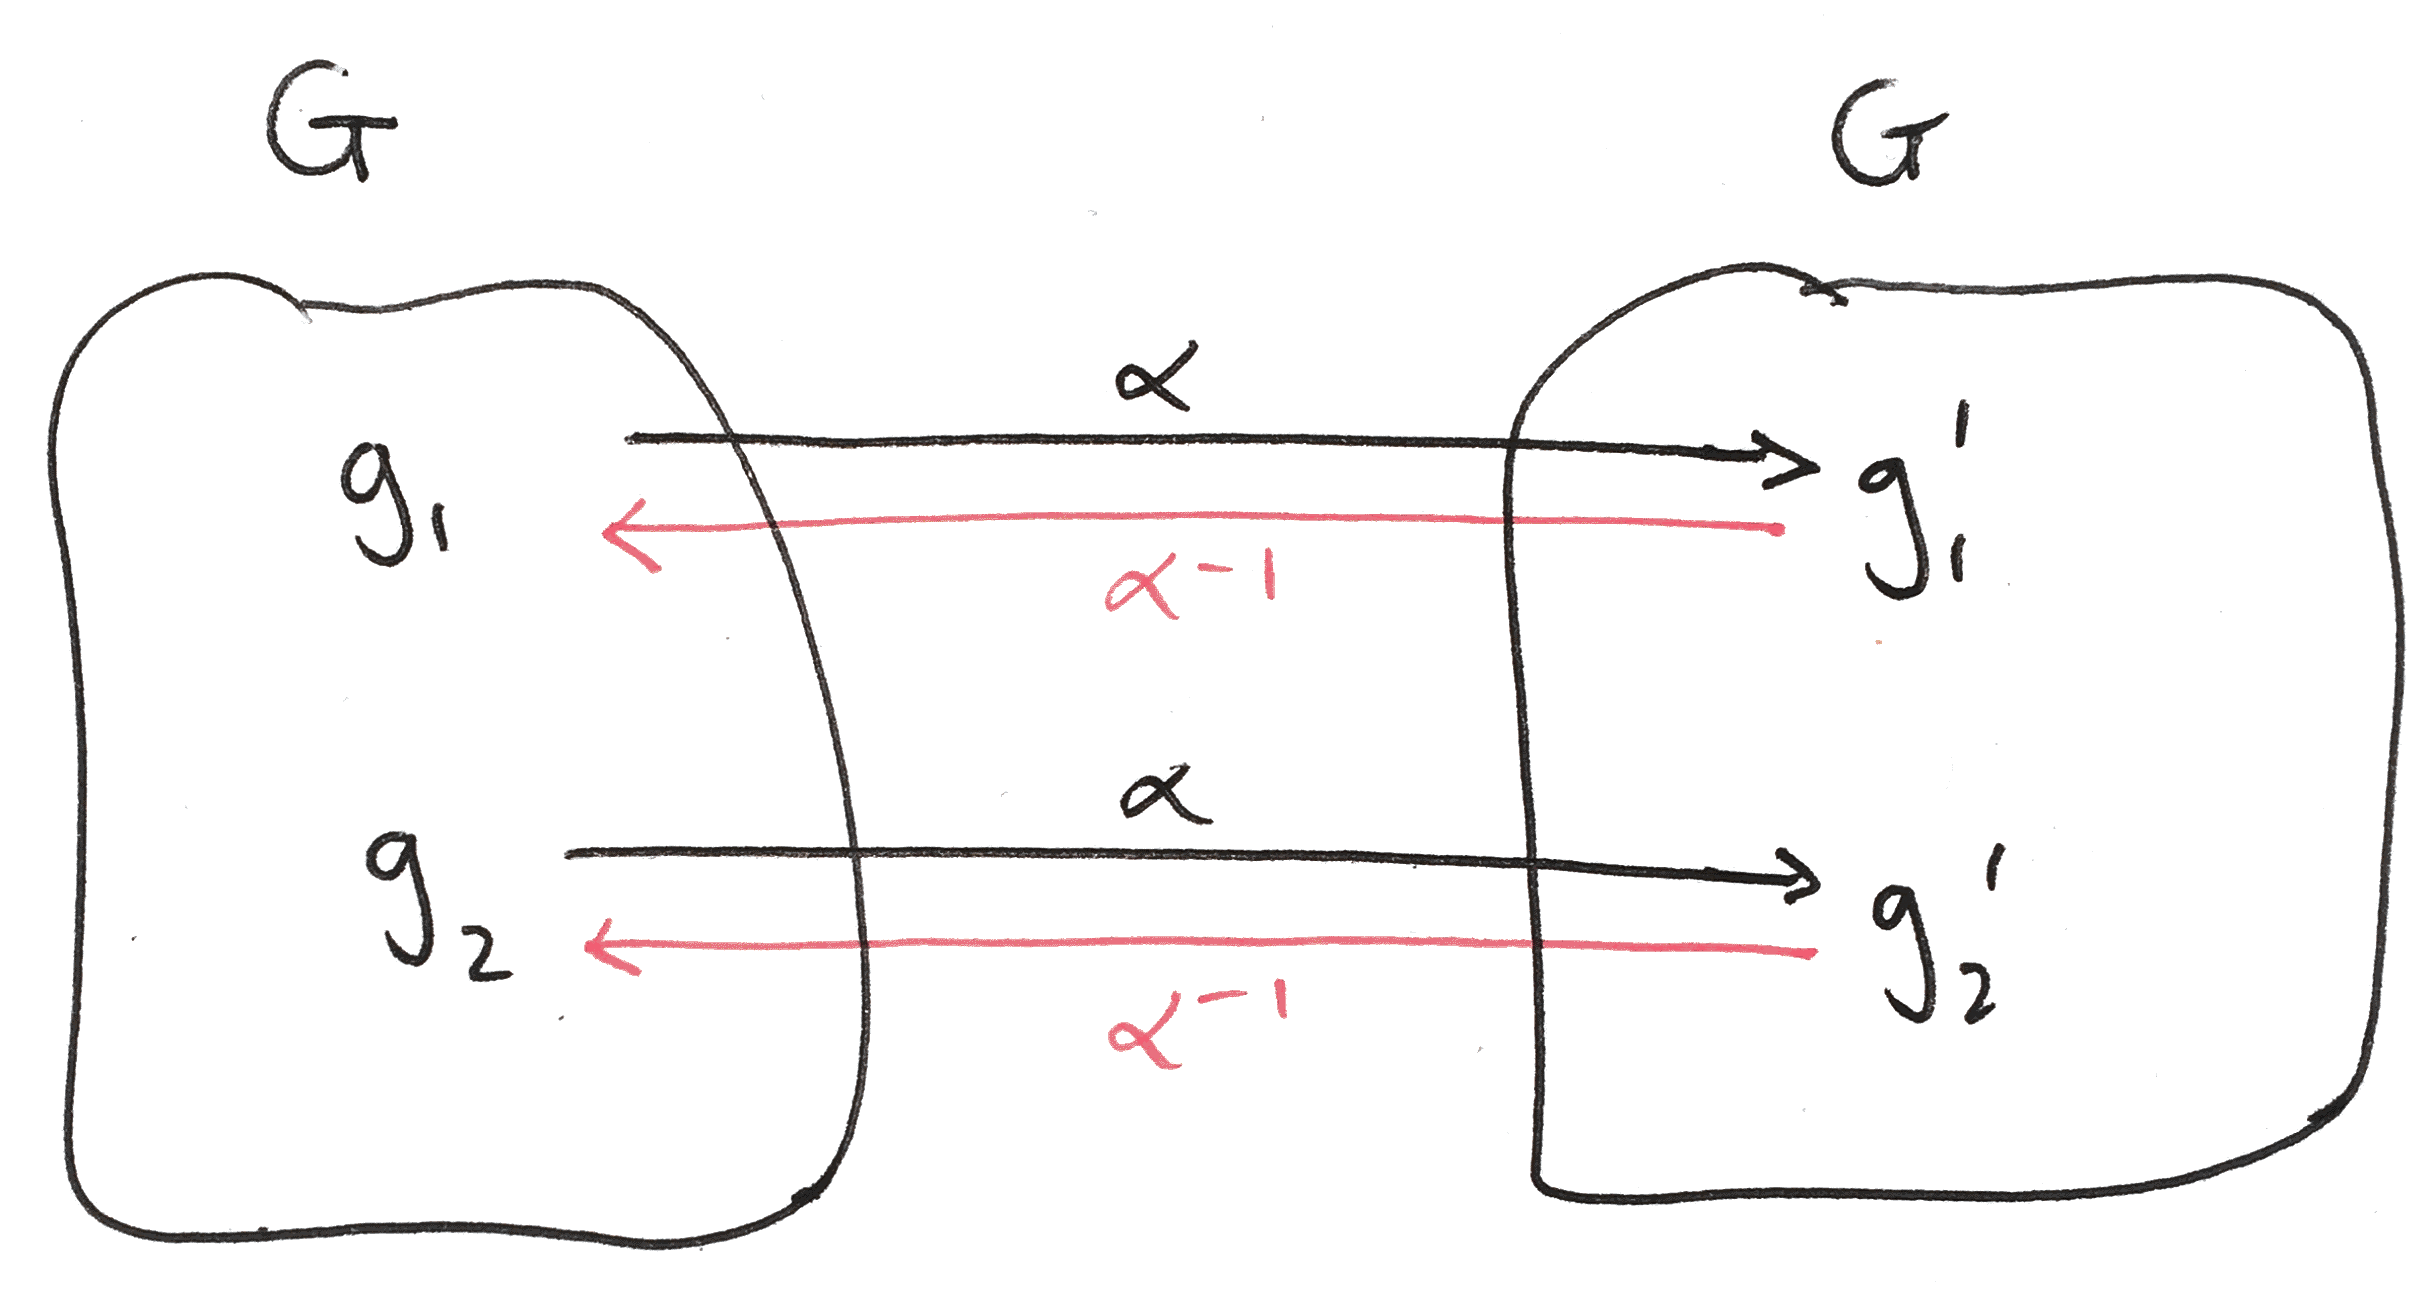
\includegraphics[width=300pt]{img/inverse-of-automorphism-1.png}
\end{mdframed}

We need to show that $\alphainv$ preserves structure, i.e. that when $\alphainv$ acts
on an element which is a product, say $g_1'g_2'$, it sends it to the product of
whatever it send the individual factors to:

$$
\alphainv(g_1'g_2') = \alphainv(g_1')\alphainv(g_2').
$$


Firstly, we know that $\alphainv(g_1')$ and $\alphainv(g_2')$ exist, i.e. some elements
are taken to them by $a$, because $a$ is an automorphism and therefore
surjective. So we'll call those $g_1$ and $g_2$, and the equality we need to
demonstrate has become

$$
\alphainv(\alpha(g_1)\alpha(g_2)) = g_1g_2.
$$

Since $\alpha$ is an automorphism, it preserves structure, therefore
$\alpha(g_1)\alpha(g_2) = \alpha(g_1g_2)$. So,

$$
\alphainv(\alpha(g_1)\alpha(g_2)) = \alphainv(\alpha(g_1g_2)) = g_1g_2,
$$

as required.
\newcommand{\textstack}[2]{
  \left(\begin{array}{c}
    \text{#1}  \\
    \text{#2}
  \end{array}\right)
}

\section{Quotient groups}

\subsection{Quotient groups and the first isomorphism theorem in plain English}
\begin{enumerate}
\item You have groups $G$ and $H$ and a homomorphism $f:G \to H$. That is special; it is not just
  any map.
\item You use the values of $f$ to define an equivalence relation $\sim$ on $G$. That's not
  special, you could do that with any map.
\item Note that this will only be interesting if $f$ is non-injective, i.e. if the equivalence
  relation does actually group some elements together.
\item You define a group operation on the equivalence classes of $G$. This is ``inherited from the
  underlying group''\footnote{ What this means is that the rule for combining equivalence classes
    is as follows:
  \begin{enumerate}
  \item Pick an arbitrary element of each equivalence class.
  \item Combine those two elements according to the group operation.
  \item Declare the result of the operation on equivalence classes to be the equivalence class of
    the group-element level result.
  \end{enumerate}
}.

So far everything has been straightforward; here is the only subtle point:

It is essential that the operation defined on the equivalence classes is well-defined. Fortunately,
it will be. Ultimately, the reason is that the equivalence classes were defined by the values of a
homomorphism, not just any arbitrary labeling.
\item So now you have a new group $G/{\sim}$ containing equivalence classes. There are four
  interesting things about it:
  \begin{enumerate}
  \item Obvious: It is smaller (simpler) than the original group $G$: you have ``modded out'' by
    the equivalence relation.
  \item Somewhat obvious: All information about the original group structure on $G$ is preserved in
    the group structure on $G/{\sim}$. This is because we decided that the group operation on the
    equivalence classes would be inherited from $G$.
  \item Obvious: There is a one-to-one correspondence between the equivalence classes and the image
    of the homomorphism (the elements of the image ``label'' the equivalence classes).
  \item Somewhat obvious: this one-to-one correspondence is actually an isomorphism.

    Why? We started off with a non-injective homomorphism $G \to H$. Then we did two things: (1) we
    coalesced into a single new element all the elements in $G$ that mapped to the same element in
    $H$; (2) we declared that the new coalesced element on the left
  \end{enumerate}
\end{enumerate}

\newpage
\begin{theorem}[First Isomorphism theorem: statement I]~\\
  Let $f:G \to H$ be a group homomorphism.

  Let $\sim$ be the equivalence relation on $G$ defined by $g_1 \sim g_2 \iff f(g_1) = f(g_2)$.

  Then the set $G/{\sim}$ of equivalence classes ``inherits the structure'' of $G$ in the following
  sense:

  Let $C_1, C_2 \in G/{\sim}$ be equivalence classes with $g_1 \in C_1$ and $g_2 \in C_2$. Define
  $C_1C_2 := $ (equivalence class of $g_1g_2$). Then this is well-defined and $G/{\sim}$ is a group
  under this operation.

  \red{TODO: state something about isomorphism of $G/{\sim}$ and $\Im f$. The group operation in
    $H$ could be anything; all we know is that $f:G \to H$ is a homomorphism. And the group
    operation in $G/{\sim}$ is inherited from $G$. The point here is that the map
    $G/{\sim} \to \Im f$ is a homomorphism, just as the original map $f:G\to H$ was. In fact, it's
    an isomorphism, because it is a bijection.}
\end{theorem}

\begin{remark*}~\\
  Note that the equivalence class of $g_1$, i.e. the preimage of $f(g_1)$, is
  \begin{align*}
    f^\1(f(g_1)) = g_1\cdot\Ker f.
  \end{align*}
  This is true since, (reverse direction) if $k \in \Ker f$, then $f(g_1k) = f(g_1)e = f(g_1)$; and
  (forwards direction) if $f(g_2) = f(g_1)$ then (\red{TODO: prove subset in this direction}).

  Therefore an equivalent definition of the equivalence relation is:

  $G/{\Ker f} := G/{\sim}$, where $g_1 \sim g_2 \iff (g_1\cdot \Ker f) = (g_2\cdot \Ker f)$.

  $G/{\Ker f}$ is a set of cosets of $\Ker f$, and may also be thought of as a set of equivalence
  classes of $\sim$.

  This gives rise to the conventional statement of the theorem:
\end{remark*}

\begin{theorem}[First Isomorphism theorem: statement II]~\\
  Let $f:G \to H$ be a group homomorphism.

  Then the set $G/{\Ker f}$ ``inherits the structure'' of $G$ in the following sense:

  Let $C_1, C_2 \in G/{\Ker f}$ be cosets of $\Ker f$, with $g_1 \in C_1$ and $g_2 \in C_2$. Define
  $C_1C_2 := $ ($g_1g_2\cdot \Ker f$). Then this is well-defined and $G/{\Ker f}$ is a group under
  this operation.

  \red{TODO: state something about isomorphism of $G/{\Ker f}$ and $\Im f$.}
\end{theorem}




\subsection{Summary}
A quotient group can be formed by:
\begin{enumerate}
\item Identify a subgroup
\item Form cosets
\item Inherit operation on cosets from operation on original group elements
\end{enumerate}
But only if the subgroup is normal: that's what's required for inheriting the group operation to
result in a well-defined operation on the cosets (i.e. when performing an operation involving
members of two different cosets, all choices of members to act as exemplars of the cosets give the
same result.)

\subsection{Modular arithmetic}

The canonical example of a quotient group comes from "modular arithmetic" on
the integers. For example, consider the integers, mod 4. This means that every
integer is mapped to whatever its remainder is after dividing by 4. The
integers mod 4 is a group, which contains 4 elements: $\{\bar 0, \bar 1, \bar
2, \bar 3\}$. So $5 \rightarrow \bar 1$, $14 \rightarrow \bar 2$, $-1
\rightarrow \bar 3$, etc.

We said that the integers mod 4 are a group, so what is the group operation?
The answer is that we define an addition law on the elements: for example,
$\bar 1 + \bar 3 = \bar{1 + 3} = \bar 4 = \bar 0$. In words, to find the result
of combining $\bar 1$ with $\bar 3$, you first add $1$ and $3$ as usual to get
4, then see where $4$ is mapped to, and that's the answer. This corresponds to
the fairly familiar notion that e.g. $5 + 23 = 28 = 0$ (mod 4), but it is a bit
subtle/slippery, and it helps to pause and consider exactly what's going on.

Let's be explicit about what $\bar 1$ actually is: it's the set of all integers
that have $1$ as their remainder when divided by $4$. So, $5 \in \bar 1$ for
example. What we've just done is define an addition operation on these
\emph{sets} (as opposed to addition of integers). The operation works as
follows. To add $\bar 2$ and $\bar 3$, you do the following:

1. Take any number that has remainder $2$ (mod $4$) and any number that has
   remainder $3$ (mod $4$).
2. Add them together using normal integer addition and find the remainder (mod
   $4$) of the result.

There are two important points here.

Firstly, we didn't need anything beyond what we had to come up with this
operation: it uses the addition operation that's \emph{already defined} on the
main group to define an operation on the subsets.

Secondly, it is only well-defined if you always get the same answer regardless
of which integers you pick in step (1). In this case that is true.

So we have an example of a ``quotient group'': $\{\bar 0, \bar 1, \bar 2, \bar
3\}$ under this addition operation. Let's recap and start putting this in group
theoretic terminology.

\footnotetext{Multiplication preserves structure also: $\Z/n\Z$ is a field iff
  $n$ is prime.}

\subsection{A quotient group is a group of cosets}

$\bar 0$ (mod $4$) is the following subset of the integers $\Z$ under addition:
$\{\ldots, -12, -8, -4, 0, 4, 8, 12, \ldots\}$. It's not only a subset, but a
\emph{subgroup} (it contains the identity element $0$, every element has an
additive inverse, and addition stays within the subset). It is written as $4\Z$
(or in general, $n\Z$ for mod $n$). However, we will often use $H$ for a
subgroup, so let's call it $H$.

$\bar 1 = \{\ldots, -11, -7, -3, 1, 5, 9, 13, \ldots\}$ is not a subgroup of
$\Z$ because it does not contain the identity element. What it is is a
\emph{coset} of the subgroup $H$: the set comprising all the results you get by
adding $1$ to elements of $H$. We can write this as $1 + H$. In fact, it's
usually written $1H$; we just have to remember that the operation here is
additive rather than multiplicative.

Of course, $\bar 2$ and $\bar 3$ are cosets defined in the same way. $\{\bar 0,
\bar 1, \bar 2, \bar 3\}$ are the only distinct cosets: for example, $\bar 4 =
4+H$ is exactly the same set of integers as $\bar 0$. Similarly, $5 + H = \bar
1$, etc.

So we arrived at the (integers mod $4$) quotient group as follows:

\begin{enumerate}
\item We started with the group of integers under addition, $\Z^+$.
\item We identified a subgroup $H$.
\item We identified the cosets of $H$: $\{H, 1+H, 2+H, 3+H\}$
\item We defined an operation on the cosets: $(i+H) + (j+H) = (i+j)+H$.
\item We noted that it was only well-defined because
  \begin{align*}
    \textstack{any number with}{remainder $i$} +
    \textstack{any number with}{remainder $j$} =
    \textstack{a number with the same}{remainder as $i+j$}.
  \end{align*}
\end{enumerate}

Note that (3) and (4) can equally be written like this, which is how it's
likely to be written when considering subgroups and cosets more abstractly:

\begin{enumerate}
\item We identified the cosets of $H$: $\{H, 1H, 2H, 3H\}$
\item We defined an operation on the cosets: $(iH) + (jH) = (ij)H$.
\end{enumerate}

\subsection{Notational digression}

The integers mod $4$ is written $\Z/4\Z$. It's an example of a quotient
group. You read that as $(\text{some group}) / (\text{some subgroup})$. In this
case the group is the integers under addition, and the subgroup is
$4Z = \{\ldots, -12, -8, -4, 0, 4, 8, 12, \ldots\}$\footnote{In this context,
  $4\Z$ always means multiplication, even if the group operation is addition!
  So it's the set $\{4z|z \in \Z\}$. It is \emph{not} the same as the coset
  $4 + \Z = \{4+z|z \in \Z\}$. This is a well-established notational
  inconsistency.}. In general, one writes $G/H$ to refer to the quotient group
of "$G$ mod $H$".


\subsection{A second example of a quotient group}

Here's an example of a (simple) problem from an undergraduate textbook on group theory:\\

\begin{mdframed}
  Identify the quotient group $\R^\times/P$, where $P$ denotes the subgroup of
  positive real numbers.
\end{mdframed}

What does this mean and how does one do it? Well, let's try to follow the same
steps as for the integers mod $4$ example above.

Our starting group is the non-zero real numbers under multiplication $\Rx$:
this plays the role of $\Z^+$ in the modular arithmetic example. And the
subgroup is the positive real numbers $P$.

What are the cosets of $P$? To get one example of a coset, you pick a number
$x$ from the main group, and you form a set by combining $x$ with each element
of the subgroup $P$ in turn. So that's the set $\{xp|p \in P\}$. We can see
that we're either going to get all the positive reals (if $x$ is positive), or
all the negative reals (if $x$ is negative). So the set of cosets has those two
sets as its elements: $\{P, -1P\}$.

OK, so we've done steps (1)-(3). Now, what's the group operation that's going
to combine two cosets and produce another coset? Well, the whole point is that
this group operation is inherited from the original group: that's what we did
in the integers mod $4$ example; we used the standard addition of integers to
define the result of adding cosets $i+H$ and $j+H$ to be the coset
$(i+j)+H$. The analogous definition here would be to use the standard
multiplication of real numbers to say that $(xP)(yP) = (xy)P$. That's going to
lead us to the following intuitively reasonable multiplication table:

$$
\begin{array}{ c|cc }
 ~   & P   & -1P \\
 \hline
 P   & P   & -1P \\
 -1P & -1P & P \\
\end{array}
$$

And we conclude that the quotient group is isomorphic to the group of size 2
(there's only one -- the one with this multiplication table).

The only question is (5): is the operation on cosets well-defined? In this
case, the answer is yes: for example, any positive number $x \in P$, multiplied
by any negative number $y \in -1P$, is going to give a negative number $xy \in
-1P$.\footnote{We can prove it easily here because the group is commutative:
$(xP)(yP) = (Px)(yP) = P(xy)P = (xy)PP = (xy)P$. In addition to commutativity
those steps make use of associativity and closure.}.


\subsection{Quotient groups of arbitrary groups}

What about in general? If we have a subgroup, can we just identify the cosets
of the subgroup, and define a composition law on them using the composition law
from the main group? Will it always be well-defined in the sense answered
above? The answer is: yes if and only if the subgroup is ``normal''.

A normal subgroup $H$ is defined to be a subgroup that is closed under
conjugation. This means that you can take any element $g$ of the main group,
form the product $ghg^\1$ using any element $h$ of the subgroup, and the result
will always be in the subgroup. One can prove that if and only if this is true,
then the composition of cosets is well-defined, in which case the prescription
above for forming a quotient group can be followed (find the cosets of $H$,
define the operation on the cosets).

So, if you need to find a quotient group of some subgroup, you need to show
that the subgroup is normal. There are two ways of doing that:

\begin{enumerate}
\item Show that it is closed under conjugation.
\item Show that it is the kernel of a homomorphism.
\end{enumerate}

\newpage
\subsection{Quotient groups}
\footnotetext{Notes based on Tim Gowers' blog \url{https://gowers.wordpress.com/2011/11/20/normal-subgroups-and-quotient-groups/}}

A mapping $f$ \underline{preserves structure} if, for example:
\begin{align*}
  a  & \mapsto f(a)\\
  b  & \mapsto f(b)\\
  ab & \mapsto f(a)f(b)
\end{align*}

An \underline{isomorphism} is a bijection that preserves structure.

A \underline{homomorphism} is a mapping that preserves structure but isn't
necessarily a bijection.\footnote{I.e. it might not be injective (might send
  different inputs to the same output), or might not be surjective (might fail
  to hit certain elements).}

\begin{theorem}
The \underline{kernel} of a homomorphism is a \underline{subgroup} \footnote{\textbf{Proof.}\\Kernel
  is $\{a:f(a) = e\}$.\\
Contains identity? Yes, homomorphisms always send the identity to the identity
($f(ea) = f(e)f(a)$ but this must equal $f(a)$, hence $f(e)$ is the identity.)
Contains inverses? Yes, $f(aa^\1) = f(a)f(a^\1) = ef(a^\1) = e$, so $f(a^\1)$ must also be $e$.}.
\end{theorem}

\textbf{Example}: the group of \emph{rotations} of $\R^3$ is a subgroup of the
group of rigid motions that fix the origin (the latter includes
reflections). Now the $\det:\GLR{3} \to \R$ mapping is a homomorphism, since
$\det(T_1T_2) \equiv \det(T1)\det(T_2)$. The rotations are those mappings with
determinant 1, hence they are the kernel of a homomorphism.

\begin{theorem}
Some subgroups are not the kernel of any homomorphism
\end{theorem}

The counter example given in the proof (below) is an element of the form
$g^\1hg$ for $h$ in the subgroup and $g$ outside the subgroup. Basically, we
observe that
\begin{align*}
\varphi(g^\1hg) =
\varphi(g^\1)\cdot\varphi(h)\cdot \varphi(g) =
\varphi(g^\1)\cdot e\cdot\varphi(g) =
\varphi(g^\1)\cdot \varphi(g) =
\varphi(e) =
e,
\end{align*}
and therefore that the subgroup, if it is to be a kernel, must \emph{contain}
all products of the form $g^\1hg$ (conjugation by an element outside the
subgroup).

So,
\begin{align*}
  \textbf{kernel of homomorphism} \implies \textbf{closed under conjugation}.
\end{align*}
But does
\begin{align*}
  \textbf{closed under conjugation} \implies \textbf{kernel of homomorphism} ~ ?
\end{align*}
Yes. Closure under conjugation implies that the \textbf{subgroup is the kernel
  of the homomorphism which maps $g$ to its coset, with the operation on cosets
  inherited from the group}: $(g_1H) \cdot (g_2H) = g_1g_2H$. Justification of
this claim follows.

Suppose that $\varphi:G \to K$ is a homomorphism from $G$ to some group $K$,
and that the kernel of $\varphi$ is $H$ and that $H$ is closed under
conjugation. What can we deduce about $\varphi$?

\begin{theorem}~\\
  The left and right cosets of $H$ coincide, and $\varphi$ is constant on
  the cosets, taking different values on each coset.
\end{theorem}

This means that there is a \underline{bijection} between the cosets of $H$ and
the \underline{image} of $\varphi$. So, we can say that the image of $\varphi$
\textit{is} the cosets of $H$.

\begin{theorem}~\\
  If $\varphi(g_1H) = a_1$ and $\varphi(g_2H) = a_2$ then
  $\varphi(g_1g_2H) = a_1a_2$.
\end{theorem}

This allows us to define the group operation on the elements of the image of
$\varphi$: it implies that
\begin{align*}
  (g_1H) \cdot (g_2H) = g_1g_2H.
\end{align*}

\begin{theorem}
\begin{align*}
  \textbf{kernel of homomorphism} \iff \textbf{closed under conjugation} \iff gH = Hg ~~~ \forall g \in G
\end{align*}
\end{theorem}

~\\~\\~\\~\\~\\
\hrule
\begin{theorem*}
  Some subgroups are not the kernel of any homomorphism.
\end{theorem*}

\begin{proof} \label{some-subgroups-not-kernel}
Counter-example: consider the permutation group
$S_3 = \{e, (12), (13), (23), (231), (312)\}$, and its subgroup $\{e,
(12)\}$.

Suppose this subgroup is the kernel of a homomorphism. I.e.
$e \mapsto e, (12) \mapsto e$, but nothing else is sent to the identity.

Now consider $(13)(12)(13)$:
\begin{align*}
  123 \to 321 \to 231 \to 132,
\end{align*}
i.e. $(13)(12)(13) = (23)$.

But
\begin{align*}
  \varphi\Big((13)(12)(13)\Big) =
  \varphi\Big((13)\Big) \varphi\Big((12)\Big) \varphi\Big((13)\Big) =
  \varphi\Big((13)\Big) \varphi\Big((13)\Big) = \varphi\Big((13)(13)\Big) = e,
\end{align*}
so $(23) \mapsto e$, which is a contradiction. Therefore $\{e,(12)\}$ isn't the
kernel of any homomorphism.
\end{proof}

\begin{theorem*}
  The left and right cosets of $H$ coincide, and $\varphi$ is constant on the
  cosets, taking different values on each coset.
\end{theorem*}

\begin{proof}
  TODO
\end{proof}


\begin{theorem*}~\\
  If $\varphi(g_1H) = a_1$ and $\varphi(g_2H) = a_2$ then
  $\varphi(g_1g_2H) = a_1a_2$.
\end{theorem*}

\begin{proof}
  TODO
\end{proof}
\newpage
\subsection{First isomorphism theorem}

\footnotetext{\url{https://theoremoftheweek.wordpress.com/2010/05/20/theorem-26-the-first-isomorphism-theorem/}}

Every normal subgroup is the kernel of the homomorphism that sends a group element to its coset.

Can two distinct homomorphisms share the same kernel?

Let $f: G \rightarrow G'$ be a homomorphism with kernel $N$. $e \in N$,
therefore every $g \in G$ is in some coset $gN$, so the set of cosets
partitions the domain. What about the image? Consider two elements $gn_1$ and
$gn_2$ of the same coset. These both get sent to the same value, since
$f(gn_i) = f(g)f(n_i) = f(g)$.

So is it possible to have homomorphisms $f$ and $\varphi$ with the same kernel
$N$ but with $f(g) \neq \varphi(g)$ for some $g \in G$? If that were true [...]
\section{Exercises - Harvard E122}
Exercises from Artin *Algebra* 1st edition.

\begin{itemize}
\item [Harvard E122](http://wayback.archive-it.org/3671/20150528171650/https://www.extension.harvard.edu/open-learning-initiative/abstract-algebra)
\item [Harvard 122](http://www.math.harvard.edu/~ctm/home/text/class/harvard/122/02/html/hw.html)
\end{itemize}

\hrule

\subsection{E122 Homework 1}

** 1. Read 1.1, pp. 38-42 **

** 1.1.7 Find a formula for $\smatt{1}{1}{1}
                                   { }{1}{1}
                                   { }{ }{1}^n$ and prove it by induction. **

** 1.1.16 **

** 1.1.17 **

\hrule
\subsection{E122 Homework 2}
**Read 2.1, 2.2**

** 2.1.5 **

** 2.1.7 **

** 2.2.1 **

** 2.2.14 (122) Let $G$ be a cyclic group of order $n$, and let $r$ be an integer
dividing $n$. Prove that $G$ contains exactly one subgroup of order $r$. **

If $n$ is prime then the only subgroups of $G$ are $\{e\}$ and $G$. The
integers which divide $n$ are 1 and $n$ and so it is true that for every such
integer $r$ there is one subgroup of order $r$.

If $n$ is not prime then $G$ has non-trivial subgroups for every integer that
divides it.

For example, if $G$ has order 8, the claim is that $G$ has only one subgroup of
order 2. Well, all subgroups of order 2 are isomorphic to $\{e, \tau\}$. So the
claim implies that groups of permutations of order 4, 6, 8 etc (i.e. $S_4, S_6,
S_8$) contain only one transposition.


A solution is given in the
[Harvard 122 materials](http://www.math.harvard.edu/~ctm/home/text/class/harvard/122/02/html/home/solns/hw2.pdf).

The starting point is to note that $<g^{n/r}>$ is a subgroup of order $r$
($n/r$ fits $r$ times into each chunk of $n$ items). So in the example with $G$
of order 8, $<g^{4}>$ has order 2. The question is whether there is any other
subgroup of order 2. Intuitively it seems obvious that the answer is no, since
only 4 divides up chunks of 8 in that way.

Formally, the proof proceeds by supposing that $H' = <g^m>$ also has order $r$
(using a lemma that every subgroup of a cyclic group is cyclic). It then shows
that $m$ must divide $n$ (otherwise leads to a contradiction). Therefore the
order of $H'$ is $n/m$. Therefore $m = n/r$ which shows that $H'$ is $H$.

** 2.2.15 **

** 2.2.20(a) **


\hrule

\subsection{E122 Homework 3}

** 2.3.1 **

** 2.3.11 **

** 2.3.12 **

** 2.4.3 **

** 2.4.5 (122) **

** 2.4.6 **

** 2.4.8 (122) **

** 2.4.11 **

** 2.4.16 (122) **

** 2.4.23 (122) **


\hrule
\subsection{E122 Homework 4}
** 1. Read Artin 1.4.**

** 2. Let $V$ denote the Klein 4-group. Show that Aut($V$) is isomorphic to $S_3$.**

Every automorphism sends the identity to itself. This is because an
automorphism must preserve structure, therefore we require $\rho(e) =
\rho(ee^\1) = \rho(e)\rho(e^\1) = \rho(e)\rho(e)^\1$ which implies $\rho(e) =
e$.

Therefore, elements of Aut($V$) are distinguished by their effect on the 3
non-identity elements and there is a 1-1 correspondence $f$ between elements of
Aut($V$) and $S_3$.

We need to show that $f$ is a homomorphism, i.e. that $f(\rho_1 \rho_2) =
f(\rho_1) f(\rho_2)$. The operation is composition of permutations in both
groups...the identity seems obvious.

**3.**

Define $f : \GL_n(\R) \rightarrow \GL_n(\R)$ by $f(A) =~ ^tA^\1$ (where $^tA$
is the transpose of $A$). Show that $f$ is an automorphism, but not an inner
automorphism for $n ≥ 1$.

To show that $f$ is an automorphism we need to show that it preserves structure
and is a bijection.

*Preservation of structure:* We require that $^t(AB)^\1 =~ ^tA^\1~ ^tB^\1$.
The RHS is $^tA^\1~ ^tB^\1 = (^tB^tA)^\1 = ~^t(AB)^\1$ as required.

*Bijection:* $f^\1(A) =~ ^tA$. Since an inverse mapping exists, the original
mapping must be bijective.

Finally, we need to show that $f$ is not an inner automorphism for $n \geq
1$. An inner automorphism is an automorphism defined by $\rho(A) = BAB^\1$ for
some fixed $B$. So we need to show that there is no $B$ for which $^tA^\1 =
BAB^\1$ for all $A$. $BAB^\1$ corresponds to the action of $A$ performed in a
basis defined by $B$. The determinant of $A$ is invariant under change of
basis. However, $\det ~^tA^\1 = (\det A)^\1$. Therefore $^tA^\1 = BAB^\1$ is
not true in general since it is not true when $\det A \neq \pm 1$.

http://math.stackexchange.com/questions/98378/fx-tx-1-is-an-automorphism-of-gl-n-mathbbr

I'm also watching these lectures and trying to do the homework, so by no means
an expert. In the final part of the proof, a variant would be to use
determinants:

Assume that $f$ is an inner automorphism. Therefore for some fixed $B$, $^tA^\1
= BAB^\1$ for all $A$. But this implies $(\det A)^\1 = \det A$ which is true
only for $\det A = \pm 1$. Therefore $f$ is not an inner automorphism.


**4. 1.4.5 Prove that the transpose of a permutation matrix P is its inverse.**

\subsection{E122 Homework 5}
\hrule

**2.5.1 Prove that the nonempty fibres of a map form a partition of the domain.**

We need to show

1. That every element of the domain is in some fibre, and
2. That no element is in more than one fibre

Let $f$ be a map from set $S$ to set $T$. A fibre $\phi_t$ of $f$ is the set
$\{s: f(s) = t\}$.

For any element $s$ in the domain, $f(s)$ exists and $s$ is in fibre
$\phi_{f(s)}$. This proves (1).

To prove (2), suppose that $s$ belongs to fibres $\phi_{t_1}$ and
$\phi_{t_2}$. Then $f(s) = t_1$ and $f(s) = t_2$ which is a contradiction
showing that no element belongs to two fibres.

\hrule

**2.5.6**

**(a) Prove that the relation $x$ conjugate to $y$ in a group $G$ is an
  equivalence relation on $G$.**

$x$ conjugate to $y$ means $y = gxg^{-1}$ for some $g \in G$. We need to show
that the relation is reflexive, transitive and symmetric.

*Reflexivity*: $x$ is equal to $x$ conjugated with the identity element: $x = exe^{-1}$.

*Symmetry*: Let $y = gxg^{-1}$. Then multiplying on the right by $g$ and on the
            left by $g^{-1}$ gives $g^{-1}yg = x$.

*Transitivity*: Let $y = g_1xg_1^{-1}$ and $z = g_2yg_2^{-1}$. Then $z =
                g_2(g_1xg_1^{-1})g_2^{-1} = (g_2g_1)x(g_1^{-1}g_2^{-1})$


**(b) Describe the elements $a$ whose conjugacy class (= equivalence class)
consists of the element $a$ alone.**

\hrule

**2.6.2 Prove directly that distinct cosets do not overlap.**

Let $H$ be a subgroup of $G$ and let $g_1H = \{g_1h:h\in H\}$ be a coset of $H$
in $G$. Consider an element $g_3 \in g_1H$. This means that $g_3 = g_1h$ for a
unique $h \in H$.

Suppose that $g_3$ is also in another coset $g_2H$. Then $g_3 = g_1h = g_2h'$
for $h, h' \in H$ and therefore $g_1hh'^{-1} = g_2$. But $hh'^{-1} \in H$ so
$g_2$ is in coset $g_1H$, which shows that cosets $g_1H$ and $g_2H$ are the
same.

\hrule

**2.6.4 Give an example showing that left cosets and right cosets of $\GL_2(\R)$
  in $\GL_2(\C)$ are not always equal.**

We don't even need to consider matrices outside $\GL_2(\R)$. Let A =
$\smat{1}{0}
      {0}{0}$ and let $H = \GL_2(\R)$.

Geometrically, this matrix projects points in 2D onto the x-axis.

The left coset of $\GL_2(\R)$ containing $A$ is the set of matrices of the form

$$
\smat{1}{0}
     {0}{0} \smat{a}{b}
                 {c}{d} = \smat{a}{b}
                               {0}{0}
$$

where $a,b,c,d \in \R$. Geometrically, this composition first sends the basis
vectors to new locations with x-coordinates $a$ and $b$, and then projects onto
the x axis.

The right coset of $\GL_2(\R)$ containing $A$ is the set of matrices of the form

$$
\smat{a}{b}
     {c}{d} \smat{1}{0}
                 {0}{0} = \smat{a}{0}
                               {c}{0}
$$

Geometrically, this composition first sends the $\scvec{0}{1}$ basis vector to
the origin, and then performs an arbitrary linear transformation. But once sent
to the origin, the $\scvec{0}{1}$ basis vector stays there, regardless of the
nature of the second transformation.

\hrule

**2.6.5 Let $H$, $K$ be subgroups of a group $G$ of orders 3, 5
  respectively. Prove that $H \cap K = \{e\}$.**

Since $H$ and $K$ are of prime order, they are isomorphic to the cyclic groups
of orders 3 and 5 respectively. Therefore the non-identity elements of $H$ are
of order 3, and the non-identity elements of $K$ are of order 5 (because the
order of an element in a group must divide the order of the group). Therefore,
while $e$ is in $H \cap K$, no other element is.

\hrule


** 2.6.10 (122) **

** 2.6.11 (122) **

** 2.8.2 (122) **

** 2.8.10 (122) **


\subsection{E122 Homework 6}

\hrule
** 2.9.2 2. **

** (a) Prove that the square $a^2$ of an integer $a$ is congruent to 0 or 1 modulo 4. **

Suppose $a$ is even, so $a = 2n$ for some $n \in \Z$. Then $a^2 = 4n^2 \equiv
0$ (mod 4). Alternatively, suppose $a$ is odd, i.e. $a = 2n + 1$ for some $n
\in \Z$. Then $a^2 = 4n^2 + 4n +1 \equiv 1$ (mod 4).

** (b) What are the possible values of $a^2$ modulo 8? **

If $a$ is even, then $a^2 = 4n^2$. If $n^2$ is odd then $a^2 \equiv 4$ (mod 8)
and if even then $a^2 \equiv 0$ (mod 8). If $a$ is odd, then $a^2 = 4n(n+1) + 1
\equiv 1$ (mod 8). So the possible values are 0, 1, 4.


\hrule

** 2.9.4 Prove that every integer a is congruent to the sum of its decimal
digits modulo 9. **

Let $a = d_0 + d_1 10 + d_2 10^2 + \ldots$.

[*Good solution*](https://github.com/AMouri/artin-algebra/blob/3083860baf553b472495fd01ef62489db9a261ee/Chapter%202%20-%20Groups/Section%209%20-%20Modular%20Arithmetic/solutions.tex#L47):
Note that $10 \equiv 1$ (mod 9). So $a \equiv d_0 + d_1 + d_2 + \ldots$ (mod 9).

*My solution*: we require that the difference is a multiple of 9. The difference
is $\sum_{i=0}^\infty d_i 10^i - \sum_{i=0}^\infty d_i = \sum_{i=0}^\infty
d_i(10^i - 1)$...which is a multiple of 9.


\hrule

** 2.9.5 Solve the congruence $2x \equiv 5$ **

** (a) modulo 9 **

[*Good solution*](https://github.com/AMouri/artin-algebra/blob/3083860baf553b472495fd01ef62489db9a261ee/Chapter%202%20-%20Groups/Section%209%20-%20Modular%20Arithmetic/solutions.tex#L52):
$x = 2^\1 5 \equiv 5 \cdot 5 \equiv 7$ (mod 9)

The possible values of $2x$ (mod 9) are 0, 2, 4, 6, 8, 1, 3, 5, 7, 9. So 2 (mod
9) does have a multiplicative inverse (5).


*My solution*: $14 = 2 \cdot 7 \equiv 5$ (mod 9). So the solution is $x \equiv 7$ (mod 9).

** (b) modulo 6 **
[*Good solution*](https://github.com/AMouri/artin-algebra/blob/3083860baf553b472495fd01ef62489db9a261ee/Chapter%202%20-%20Groups/Section%209%20-%20Modular%20Arithmetic/solutions.tex#L54)
The possible values of $2x$ (mod 6) are 0, 2, 4. Therefore $2x \equiv 5$ has no
solution.

I.e. 2 (mod 6) has no multiplicative inverse?

*My solution*: $\bar 5$ (mod 6) $= 5 + 6\Z = 1 + 2\cdot2 + 2\cdot3\Z = 1 + 2(2 + 3\Z)$ is an
equivalence class of odd numbers. Therefore $2x \equiv 5$ (mod 6) has no
solutions.



\hrule

**2.9.8 Use Proposition (2.6) to prove the Chinese Remainder Theorem: Let $m$,
$n$, $a$, $b$ be integers, and assume that the greatest common divisor of $m$
and $n$ is 1. Then there is an integer $x$ such that $x \equiv a$ (mod $m$)
and $x \equiv b$ (mod $n)$.**

Proposition 2.6 is the theorem describing the fact that, for two integers $i$
and $j$, $\gcd(i, j)$ generates the subgroup $i\Z + j\Z$.

Here's the proof from [A Mouri's solutions](https://github.com/AMouri/artin-algebra/blob/3083860baf553b472495fd01ef62489db9a261ee/Chapter%202%20-%20Groups/Section%209%20-%20Modular%20Arithmetic/solutions.tex#L66):

\hrule

From Proposition 2.6, $1 = an + bm$. Then

$1 \equiv an + bm$ (mod $m$) $\rightarrow 1 \equiv an$ (mod $m$).

Since $\gcd(n, m) = 1$, then $n^{-1} \equiv a \mod m$. Similarly, $m^{-1}
\equiv b \mod n$.

\hrule
My attempt:

We need to show that for any values $a,b$, we can always find an integer $x$
which exceeds the previous multiple of $m$ by $a$ and exceeds the previous
multiple of $n$ by $b$.

So we want to show that the intersection of $a + m\Z$ and $b + n\Z$ is
non-empty. I.e. we need to show that we can always find integers $r, s$
satisfying $a + rm = b +sn$. That's equivalent to $rm - sn = b - a$. We know
that $m\Z + n\Z = \gcd(m, n)\Z$, and thus since $\gcd(m, n) = 1$ we know that
$m\Z + n\Z$ is all of $\Z$. Therefore the integer $b - a$ must be reachable by
taking some number $b$ of steps of length $m$ and some number $-a$ of steps of
length $n$.

\subsection{E122 Homework 7}

\hrule


** 2.10.1 (E122 \& 122) Let $G$ be the group of invertible real upper triangular
2 x 2 matrices. Determine whether or not the following conditions describe
normal subgroups $H$ of $G$. If they do, use the First Isomorphism Theorem to
identify the quotient group $G/H$. **

$G = \left\{ \mat{a}{b}
                 {0}{d} \right\}$

** (a) $a_{11} = 1$ **

$H = \left\{ \mat{1}{b}
                 {0}{d} \right\}$

This is closed, contains the identity and contains inverses, so it is a
subgroup. And closed under conjugation, so normal.

Geometrically, the elements of the subgroup $H$ are matrices representing a
stretch in the direction of the second basis vector ("Y axis") and shearing
parallel to the first basis vector ("X axis). Conjugation yields matrices
$ghg^\1$ which correspond to doing the same transformation in a different
basis. However, this class of change-of-basis operations preserves the
direction of the first basis vector. Therefore the transformation, in the new
basis, also corresponds to stretching in the direction of the second basis
vector and shearing parallel to the first basis vector, and thus the conjugated
matrix is still in the subgroup.

\begin{align*}
&\mat{e}{f}
     {0}{h} \mat{1}{b}
                {0}{d} \mat{h}{-f}
                           {0}{e} \frac{1}{eh} \\
= &\mat{e}{f}
       {0}{h} \mat{h}{-f + be}
                  {0}{de     } \frac{1}{eh} \\
= &\mat{eh}{e(-f + be) + fde}
       {0}{hde} \frac{1}{eh}
\end{align*}


The theory of quotient groups involves identifying establishing a group
structure on a set of cosets of a normal subgroup: this set of cosets is then a
quotient group $G/H$. There's a homomorphism $f:G \rightarrow G/H$ defined by
$f(g) =$ (coset containing $g$), and the multiplication law between cosets is

(coset containing $g$) x (coset containing $g'$) = (coset containing $gg'$)

The normal subgroup is the kernel of this homomorphism, since $f(1)$ = (coset
containing $1$) = $1H$.

So we have a subgroup $H$ of the group $G$ of real upper-triangular 2x2
matrices.  We've determined that the normal subgroup is $H$, a particular
subset of real upper-triangular matrices. Each coset is therefore, for some
fixed $g \in G$, the set of matrices that can be obtained by multiplying $g$ by
some $h \in H$. So there are infinitely many cosets and each has infinitely
many elements. Each coset contains matrices of the form

\begin{align*}
\mat{1}{b}
    {0}{d} \mat{e}{f}
               {0}{h} = \mat{e}{b + df}
                            {0}{dh    }.
\end{align*}

Since $b$ and $d$ can be any real numbers, we could write this as

\begin{align*}
\mat{1}{*}
    {0}{*} \mat{a}{b}
               {0}{d} = \mat{a}{*}
                            {0}{*},
\end{align*}

thus the cosets are distinguished by the real number in their top-left
entry. So the quotient group $G/H$ is $\left\{\smat{a}{*} {0}{*}: a \in
\R\right\}$; it is isomorphic to the positive real numbers (elements of $G$
would not be invertible if $a$ were $0$). Viewed as transformations of the
plane, the elements of $G/H$ are distinguished by the magnitude of their
stretch in the x-direction.

\hrule
** (b) $a_{12} = 0$ **

$H = \left\{ \mat{a}{0}
                 {0}{d} \right\}$

This is closed, contains identity and inverses, hence is a subgroup. However
again, it is not closed under conjugation, so not normal.

Geometrically, the matrix represents a stretch in orthogonal x- and
y-directions. The non-normality is because the matrix that performs the
transformation in the changed basis does not stretch in the directions of the
basis vectors in the original basis.

\begin{align*}
&\mat{e}{f}
     {0}{h} \mat{a}{0}
                {0}{d} \mat{h}{-f}
                           {0}{e } \frac{1}{eh} \\
= &\mat{e}{f}
       {0}{h} \mat{ah}{-af}
                  {0 }{de } \frac{1}{eh} \\
= &\mat{eah}{-eaf + fde}
       {0  }{hde       } \frac{1}{eh}
\end{align*}

\hrule
** (c) $a_{11} = a_{22}$ **

$H = \left\{ \mat{a}{b}
                 {0}{a} \right\}$

Closed and contains identity and inverses, so a subgroup, but again not closed
under conjugation.

Geometrically, the matrix represents a stretch by the same amount in orthogonal
x- and y-directions, plus a shear. The non-normality is because the matrix that
performs the transformation in the changed basis does not stretch equally in
the directions of the basis vectors in the original basis.

\begin{align*}
&\mat{e}{f}
     {0}{h} \mat{a}{b}
                {0}{d} \mat{h}{-f}
                           {0}{e } \frac{1}{eh} \\
= &\mat{e}{f}
       {0}{h} \mat{ah}{-af + be}
                  {0 }{de      } \frac{1}{eh} \\
= &\mat{eah}{e(-af + be) + fde}
       {0  }{hde              } \frac{1}{eh}
\end{align*}


\hrule
** (d) $a_{11} = a_{22} = 1$ **

$H = \left\{ \mat{1}{b}
                 {0}{1} \right\}$

Closed, contains identity and inverses. It performs a shear, with no
stretching. Closed under conjugation and therefore normal.

Geometrically, the matrix represents a shear, with no stretching. The normality
is because the matrix that performs that transformation in the changed basis
also performs a shear without stretching in the original basis.


\begin{align*}
&\mat{e}{f}
     {0}{h} \mat{1}{b}
                {0}{1} \mat{h}{-f}
                           {0}{e} \frac{1}{eh} \\
= &\mat{e}{f}
       {0}{h} \mat{h}{-f + be}
                  {0}{e      } \frac{1}{eh} \\
= &\mat{eh}{e(-f + be) + fe}
       {0  }{eh             } \frac{1}{eh}
\end{align*}

Each coset contains matrices of the form

\begin{align*}
\mat{1}{b}
    {0}{1} \mat{e}{f}
               {0}{h} = \mat{e}{f + bh}
                            {0}{h     }.
\end{align*}

which could be written as

\begin{align*}
\mat{1}{*}
    {0}{1} \mat{e}{f}
               {0}{h} = \mat{e}{*}
                            {0}{h}.
\end{align*}

The elements of the quotient group $G/H$ are thus distinguished by their
diagonal entries. I.e., $G/H$ is isomorphic to $\R^2$.


\hrule

** 2.10.3 Let $P$ be a partition of a group $G$ with the property that for any
pair of elements $A, B$ of the partition, the product set $AB$ is contained
entirely within another element $C$ of the partition. Let $N$ be the element of
$P$ which contains 1. Prove that $N$ is a normal subgroup of $G$ and that $P$
is the set of its cosets. **

** Prove that $N$ is a normal subgroup of $G$: **

We know that $1 = 1^\1$ is in $N$. Therefore we know that the product set $NN$
must lie entirely within $N$, since one example of a product
(i.e. $1\cdot1^\1$) is in $N$. I.e. $N$ is closed. Does it contain inverses?
Consider an arbitrary element $n$ of $N$. Let $n^\1$ be in some element $A \in
P$ of the partition. Then the product set $NA$ must lie entirely within $N$,
since $nn^\1$ does. So either $A = N$, or $N$ and $A$ are distinct elements of
the partition but with the property that $NN = NA$. I'm going to say that $NN =
NA$ implies $N = A$ by the definition of the problem, and thus that $N$
contains inverses, but I may be missing something here.

So, $N$ contains the identity, is closed and contains inverses. It inherits
associativity from $G$. So $N$ is a subgroup. Is it normal? Consider $gNg^\1$
for some fixed $g$. Since $1 \in N$, we conclude that $gN$ is a subset of the
element $A$ of the partition that contains $g$. And since $g \in gN$,
$(gN)g^\1$ must be a subset of $N$. Therefore $N$ is normal.

** Prove that $P$ is the set of its cosets: **

The set of cosets of $N$ are $\{gN: g \in G\}$ by definition.

We need to show that exactly one partition satisfying the definition of $P$
exists, and that it is the set of cosets of $N$.

First, we show that the set of cosets satisfy the definition of $P$. Consider
two cosets $gN$ and $hN$. Their product set is $(gN)(hN)$. We know that $g \in
gN$ and $h \in hN$ so we conclude that $(gN)(hN)$ is a subset of the element of
the partition that contains $gh$.

So the set of cosets satisfy the definition of $P$, showing that at least one
such partition exists. Now we show that any such partition must be the set of
cosets. Consider subsets $A, B$ of $G$ that satisfy the definition of $P$. We
need to show that $A$ and $B$ are cosets of $N$. Fix an arbitrary element $a$
of $A$. Since $1 \in N$ and $a1 \in A$ we conclude that the product set $AN$ is
equal to $A$ and therefore that $A$ is equal to the coset $aN$. Similarly, $B$
is a coset of $N$.

\hrule

** 2.10.5 Identify the quotient group $\R^\times/P$, where $P$ denotes the subgroup of
positive real numbers. **

The cosets of $P$ are the positive and negative reals, $\{P, -1P\}$. We define
composition of cosets to be $(xP)(yP) = (xy)P$. The group operation is
commutative, therefore $P$ is normal and the operation on cosets is
well-defined. Therefore the quotient group is isomorphic to the group of size
2: $P$ is the identity and $(-1P)(-1P) = P$.

\hrule

** 2.10.6 Let $H = \{±1, ±i\}$ be the subgroup of $G = \Cx$ of fourth roots
of unity. Describe the cosets of $H$ in $G$ explicitly, and prove that $G/H$ is
isomorphic to $G$. **

The cosets of $H$ in $G$ are sets of the form $zH = \{±z, ±zi\}$, where $z \in
\Cx$. Geometrically, they are the four points of a cross in the complex
plane; a rotated and scaled version of the unit cross corresponding to $\{±1,
±i\}$.

If $z \neq z'$ then $zH \neq z'H$. So there is a bijection between $G/H$ and
$G$. I.e. $G/H$ is isomorphic to $G$.

\hrule

** 2.10.10 (122) Describe the quotient groups $\Cx / P$ and $\Cx /
U$, where $U$ is the subgroup of complex numbers of absolute value $1$ and $P$
denotes the positive reals. **

** $\Cx / P$ **

The cosets of $P$ are the set of radial lines emanating from the origin in the
complex plane. So a single coset is $e^{i\theta}P = \{pe^{i\theta} | p \in P\}$
and there is one coset for every value of $\theta \in [0, 2\pi)$. We define the
following operation on the set of cosets:
$(e^{i\theta_1}P)(e^{i\theta_2}P) = e^{i(\theta_1 + \theta_2)}P$. The group operation is commutative, therefore $P$ is normal and the operation is well-defined.

So the quotient group is isomorphic to the group of angles $[0, 2\pi)$ under addition, and to $U$. This is the "circle group" $T$.


** $\Cx / U$ **

The cosets of $U$ are concentric circles in the complex plane. So a single coset is $re^{i\phi}U = rU = \{re^{i\theta}|0\leq\theta<2\pi\}$, and there is one coset for every $r \in P$. We define the
following operation on the set of cosets: $(r_1U)(r_2U) = r_1r_2U$. The group operation is commutative, therefore $U$ is normal and the operation is well-defined.

So the quotient group is isomorphic to $P$, the positive reals under multiplication.

\subsection{E122 Homework 8}


\hrule

** 3.1.1 Which of the following subsets of the vector space of real $n \times
n$ matrices is a subspace?**

** (a) symmetric matrices ($A = A^t$) **

This is a subspace: it's closed under addition, contains the identity (zero
matrix), and contains additive inverses, and is closed under scalar
multiplication.

** (b) invertible matrices **

This is not a subspace, since the additive identity (zero matrix) is not an
invertible matrix. (It's closed under scalar multiplication but I'm not sure if
it contains additive inverses.)

** (c) upper-triangular matrices **

This is a subspace, since the additive identity (zero matrix) is upper
triangular, and it is closed under scalar multiplication and contains additive
inverses.

\hrule

** 3.1.5 Prove that the classification of subspaces of $\R^3$ stated after
(1.2) is complete **

> The subspaces of $\R^3$ are of four types
>
> (i) The zero vector
>
> (ii) Vectors lying in a line through the origin
>
> (iii) Vectors lying in a plane through the origin
>
> (iv) The whole space $\R^3$

Subspaces must contain the identity. So $\{0\}$ is one subspace. Now consider a
subspace that contains $x \neq 0$ in addition to $0$. In order to be closed
under scalar multiplication the subspace must also contain all vectors $x' =
cx$ for every $c \in \R$. So that's a line through the origin and $x$. One such
subspace exists for every distinct direction that a line through the origin can
take. Next planes...


** 3.2.1 Prove that the set of numbers of the form $a + b \sqrt 2$, where $a,
b$ are rational numbers, is a field. **

A field is by definition a set with an addition and a multiplication
operation. For each operation there must be associativity, closure,
commutativity, identity, inverses. A distributive law must hold: $(a + b)c =
ac + bc$.

More briefly, for a set $\F$ to be a field, there must be an addition law that
turns $\F$ into an Abelian group (identity $0$), and there must be a
multiplication law that turns $\F - \{0\}$ into an Abelian group (identity
$1$). Distributivity must hold: $(a + b)c = ac + bc$.

Take the **addition** operation first. Closure, commutativity and associativity
obviously hold. The identity is $0 = 0 + 0\sqrt 2$. The inverse is $(a + b
\sqrt 2)^\1 = (-a + -b \sqrt 2)$ (this is unique since the product of a
rational and irrational is irrational).

Now **multiplication**.

Closure and commutativity: $(a + b\sqrt 2)(c + d\sqrt 2) = (c + d\sqrt 2)(a +
b\sqrt 2) = (ac + 2bd) + (cb + ad)\sqrt 2$.

Associativity:
\begin{align*}
\((a + b\sqrt 2)(c + d\sqrt 2)\)(e + f\sqrt 2) = \\
\((ac + 2bd) + (cb + ad)\sqrt 2\)(e + f\sqrt 2) = \\
\((ac + 2bd)e + 2(cb + ad)f\) + \((cb + ad)e + (ac + 2bd)f\)\sqrt 2 = \\
\(ace + 2adf + 2bcf + 2bde\) + \(acf + ade + bce + 2bdf\)\sqrt 2 = \\
\end{align*}

\begin{align*}
(a + b\sqrt 2)\((c + d\sqrt 2)(e + f\sqrt 2)\) = \\
(a + b\sqrt 2)\((ce + 2df) + (cf + de)\sqrt 2\) = \\
\(a(ce + 2df) + 2b(cf + de)\) + \(a(cf + de) + b(ce + 2df)\)\sqrt 2 = \\
\(ace + 2adf + 2bcf + 2bde\) + \(acf + ade + bce + 2bdf\)\sqrt 2
\end{align*}

Identity is $1 + 0\sqrt 2 = 1$.

Inverses: $(a + b\sqrt 2)(a - b\sqrt 2) = (a^2 - 2b^2) \implies (a + b\sqrt
2)^\1 = \frac{1}{(a^2 - 2b^2)}(a - b\sqrt 2)$

Distributivity: ...bored now.

** 3.2.7 Define homomorphism of fields, and prove that every homomorphism of
fields is injective. **

A homomorphism between fields $F$ and $G$ is a function $f: F \rightarrow G$
such that $f(a+b) = f(a) + f(b)$ and $f(ab) = f(a)f(b)$.

Suppose that $f$ is not injective. Then $f(a) = f(b)$ for some $a \neq b$. So
$f(a-b) = f(a) + -f(b) = 0$. Then $f((a-b)(a-b)^\1) = f(a-b)f((a-b)^\1) = 0$
since the product of $0$ with anything is $0$; and yet $f((a-b)(a-b)^\1) = f(1)
= 1$. This is a contradiction which proves that homomorphisms must be
injective.

(So what about linear maps with non-empty nullspace / non full rank? Presumably
they are not homomorphisms?)

** 3.2.15 **

** (a) By pairing elements with their inverses, prove that the product of all
nonzero elements of $\F_p$ is $-1$. **

\begin{align*}
\prod aa^\1 bb^\1 ...
\end{align*}

** (b) Let $p$ be a prime integer. Prove Wilson's Theorem: $(p- 1)! \equiv -1$ (mod $p$). **
